\documentclass{ieeeaccess}
\usepackage{cite}
\usepackage{amsmath,amssymb,amsfonts}
\usepackage{algorithmic}
\usepackage{graphicx}
\usepackage{textcomp}
\usepackage{booktabs}
\usepackage{longtable}
\usepackage{array}
\def\BibTeX{{\rm B\kern-.05em{\sc i\kern-.025em b}\kern-.08em
    T\kern-.1667em\lower.7ex\hbox{E}\kern-.125emX}}
\begin{document}
\history{Date of publication xxxx 00, 0000, date of current version xxxx 00, 0000.}
\doi{10.1109/ACCESS.2017.DOI}

\title{Auditing Chest X-ray Classifiers for Spurious Shortcuts: Where Blind
VLM Naming Succeeds, Where It Fabricates, and What Survives the Failure}
\author{\uppercase{First A. Author}\authorrefmark{1}, \IEEEmembership{Fellow, IEEE},
\uppercase{Second B. Author\authorrefmark{2}, and Third C. Author,
Jr}.\authorrefmark{3},
\IEEEmembership{Member, IEEE}}
\address[1]{National Institute of Standards and
Technology, Boulder, CO 80305 USA (e-mail: author@boulder.nist.gov)}
\address[2]{Department of Physics, Colorado State University, Fort Collins,
CO 80523 USA (e-mail: author@lamar.colostate.edu)}
\address[3]{Electrical Engineering Department, University of Colorado, Boulder, CO
80309 USA}
\tfootnote{This paragraph of the first footnote will contain support
information, including sponsor and financial support acknowledgment. For
example, ``This work was supported in part by the U.S. Department of
Commerce under Grant BS123456.''}

\markboth
{Author \headeretal: Preparation of Papers for IEEE TRANSACTIONS and JOURNALS}
{Author \headeretal: Preparation of Papers for IEEE TRANSACTIONS and JOURNALS}

\corresp{Corresponding author: First A. Author (e-mail: author@ boulder.nist.gov).}

\begin{abstract}
High in-distribution accuracy from deep chest X-ray classifiers comes naturally alongside
reliance on spurious confounds - features which correlate with the label in training but not with the disease process itself – and fails silently should such correlation cease to hold on-site. We construct an auditor, which works through a four-step loop over a pneumothorax classifier to first detect the existence of reliance on a confound, to then localize it, to name it in clinically useful terms via a general vision-language model (VLM) without being ever informed about what to search for, and to mitigate such reliance via last layer re-training. The experiment is carried out as six validation-gated spike tests, each of which has a registered pass-fail criteria and a stop-and-report criterion. Detection and localization successfully generalize from a synthetic confound to a real device confound: we artificially introduce a dependence gap (44 percentage points on synthetic; 28.75 on real chest tubes), localize it (Grad-CAM peak-in-region 100\% synthetic; side-consistency 96.6\% real), but blind VLM naming, of course,
does not transfer. It achieves ceiling performance on the synthetic marker (precision 0.978, recall 0.90, control-
hallucination 0.02), but fails to detect the actual chest tube marker via fabrication: on tube-free control patches, the VLM hallucinates medical equipment – endotracheal tubes, central lines, catheters – at a rate of 0.55 (Llama-4-Scout) and 0.83 (Pixtral-12B) in a multi-VLM replication. This cross-model fabrication is the negative result we report, in honesty, in the center of this paper. The mitigating technique that survived the failure of VLM naming, however, did not rely on the VLM:
Deep Feature Reweighting improves worst-group (pneumothorax-without-tube) accuracy from 0.67 to 0.79 as
a 3-seed mean without degrading in-distribution
Lastly, there is a true AUC drop from US to Spain cross-site of 0.192 (95%
CI [0.159, 0.225], bootstrap), but a zero-shot test of whether
shortcircuiting the known source improves the AUC gap yields an estimate that
is essentially zero (+0.005, 95\% CI [-0.018, +0.028]) – underpowered for
ruling out even a small-to-moderate effect, but definitely not a sign of a
real improvement; it is distribution shift, which this setup cannot attribute
to the source shortcircuiting. We highlight the failure of name as the main
finding, not as a footnote, and we highlight two interpretive findings we had
to withdraw due to the falsification control.
\end{abstract}

\begin{keywords}
Chest X-ray classification, cross-site generalization, deep feature
reweighting, shortcut learning, spurious correlation, vision-language models,
VLM hallucination
\end{keywords}

\titlepgskip=-15pt

\maketitle

\section{Introduction}
\label{sec:introduction}
In-distribution accuracies of deep chest X-ray (CXR) clas-
sifiers can be very high yet focused on the features which
are correlated to the label in the training distribution but
have no causal relationship to the actual pathology: scanner
text information, laterality and positioning cues. Zech et al.
proved that the CNNs generalize worse between hospitals
than within the same hospital and can determine the origi-
nal hospital system in 99.95\%–99.98\% of cases; DeGrave,
Janizek \& Lee demonstrated that COVID-19 CXR classi-
fiers rely on the text and positioning information rather
than on the pathology itself. This type of classifier is highly
accurate yet vulnerable to distribution shift, which is prob-
lematic for patient safety since the model that relies on the
chest tube applied for treatment of a pneumothorax instead
of the pneumothorax itself is likely to give erroneous pre-
dictions exactly on the patients that do not need treatment.

Detecting this failure mode involves four steps: (1) recognizing that the classifier is using a shortcut, (2) identifying the clinical shortcut without knowing the type of shortcut in advance, (3) mitigating the use of the shortcut, and (4) demonstrating that recovery from the failure can be achieved with out-of-distribution shift. The existing literature usually deals with only one or two of the steps. Shortcut-diagnosis approaches (Zech; DeGrave; Jiménez-Sánchez et al.) recognize shortcuts based on either expert or statistical approaches, but do not automate the identification step. Generative correction approaches like RoentMod apply a correction based on the diffusion pipeline, with the downside of requiring significant generative infrastructure and fine-tuning. Worst-group robustness approaches (GroupDRO, JTT, DFR) mitigate the shortcut, but require group information to be known beforehand.
The most similar label-free identification prior art, LADDER, identifies the shortcut used by a classifier with the help of a foundation model in radiology, but requires the image to pass through a captioning model and a text-only LLM to make the detection.

The deficiency targeted by this paper is caption-less, diffusion-less, fine-tuning-less generation of names from a single pass through salient crops using a VLM with a blind prompt — not captioning nor generating captions, no diffusion nor finetuning, but directly connecting into the whole detect/localize/name/act chain and scoring against ground truth behind a control-hallucination gate: the proportion of images where the auditor names the device without a confound. This is the very identity of the design. A confound that is made up is more costly to the auditor than one that is missed, since a device that makes up shortcuts is worse than no device at all; hence the gate on precision over recall.

\subsection{Contributions}
\begin{itemize}
\item An auditor-loop for validation that detects, localizes, and
mitigates a shortcut in a pneumothorax classifier with
no labels in the target distribution, with a confound agno-
nostic core that applies to synthetic, real-device, and cross-
site scenarios from a single implementation.
\item Central discovery of the paper: The negative result, re-
ported truthfully: blind general-purpose VLM naming is
successful on a synthetic confound but unsuccessful on a
real device confound via fabrication, and this unsuccess is
a property of all models involved (both Llama-4-Scout
and Pixtral-12B fabricate devices in a majority of crops),
independently verified by HalluCXR.
\item Experiments on mechanism that show when naming fails: fabrication is not
motivated by the observability of the confound (recall cliff, not
hallucination cliff), but instead is motivated by the image and not
blind repetition--it is prior-driven overinterpretation of an ambiguous
salient area.
\item A zero-shot test on the source side of whether a known shortcut
causes a known generalization gap, without using any labels; a negative
result: the 0.192 generalization gap from US to Spain is caused by a
distribution shift that does not seem to be shortcut-based.
\item An explanation for how two interpretative findings were retracted
after running specific controls that disproved them, and presenting those
as primary results.
\end{itemize}

\section{Related Work}
\label{sec:related}
Learning shortcuts in chest radiology is already known.
Zech et al. demonstrated that CNNs generalize poorly across
hospitals than within, and identify hospital systems with
99.95 to 99.98\% accuracy. DeGrave, Janizek, \& Lee demon-
strated that COVID-19 CXR models are based on text fea-
tures and patient positioning rather than pathology. Jímenez-
Sánchez, Juodelyte, Chamberlain, \& Cheplygina provide
a manual and statistical shortcut discovery study for chest
X-rays. These studies provide evidence of the existence
of shortcuts and their danger, diagnose the shortcut learn-
ing using expert analysis and statistical associations; but do
not automate the naming process with a general model.

\textbf{Generative correction of shortcuts}. RoentMod combines a medical image generator (RoentGen) with an image-to-image editor for generation of counterfactual CXRs with certain findings, retaining their anatomy and showing discrimination improvements of 3-19\% AUC internally and 1-11\% externally, with 93\% of generated CXRs being realistic according to readers' ratings. This paper presents the most similar correction-side prior art to ours, and the approach that we directly compare against; RoentMod utilizes the pipeline for generative diffusion of an image and fine-tuning for generation of counterfactual radiographs, while our naming process makes one inference by frozen-VLM on each of 200 crops of an image without any image synthesis or any training phase whatsoever. This is indeed a tradeoff, not an improvement – the bar that RoentMod needed to pass was never set for our naming process.

\textbf{Mitigation Baselines.}  GroupDRO (Sagawa et al.,
2020) minimizes worst-group loss but relies on group la-
bels; JTT (Liu et al., 2021) amplifies the mistakes of an ERM
model to mimic group robustness without group labels;
DFR (Kirichenko et al., 2022) fine-tunes only the last
layer with group-balanced data and achieves 92.9\% and
70.1\% worst-group accuracy on Waterbirds and Civil-
Comments at much lower computational costs than GroupDRO because, it is assumed, the backbone network has learned
core features. Future work has cast doubt on whether the
last-layer fine-tuning always works; our synthetic tag experiments have demonstrated its insufficiency, showing that,
when the backbone has a pure shortcut, DFR does not recover full in-distribution performance. These methods pre-
sume that the groups are known; we attempt to learn the
groups ourselves.

\textbf{Contemporaneous work using the same shortcut}. Zhao et al.
use an autonomous coding agent pipeline involving other
things as well, that can make pneumothorax classification
with less reliance on chest drains in the datasets produced
based on NIH, achieving 60\%→31\% and 50\%→18\%
reliance decrease. The same shortcut, but a different method
of implementation (searching for agentic pipeline instead of
last-layer retraining) and a different way to measure (\%
reliance vs. worst-group accuracy and reliance gap). No
VLM-naming step, no control hallucinations measurement,
no cross-site transfer test done there either. We consider
this independent work confirming our findings contemporaneously.

\textbf{Auditing shortcuts for foundation models (closest analogues
to the naming step).} LADDER (Ghosh et al., Findings of
ACL 2025) is the closest prior art in medical imaging: it leverages
an LLM’s latent knowledge about the domain to infer the
classifier’s biases without specifying the attribute labels, and is
evaluated partly using chest X-rays. However, there are three
ways in which this is an analogy of ours, not the same thing:
(i) it analyzes the image as text (using BLIP/GPT-4o to captions + activation-to-text projection), reasoning with a text-
only LLM, whereas we input the Grad-CAM-cropped pixels
into a generic VLM that has neither captioner nor corpus;
(ii) its discovery is scored using slice Precision@10 and down
stream worst-group accuracy, without any control hallucination gate; (iii) the discovery in that work is meant to aid mitigation, meaning our failure mode of V4b would just factor
into mitigation performance. SpurLens applies GPT-4 along with open-set detectors to find
spurious signals which are over-relied upon by multimodal LLMs
in natural images and evaluates hallucination amplification (objects
hallucinated 10 times more frequently in presence of spurious cues).
RaVL uncovers region-level spurious correlations based on a fine-
tuned VLM’s own errors and mitigates using a region-aware loss
function (+8.2\% worst-group accuracy, 191\% discovery improve-
ment, 654 VLMs). Although both are close mechanism analogues,
neither of them works with medical imaging, blind clinical naming, or control-hallucination-gated metric. MIMM-X extracts the
confounding factor through mutual-information objectives, opposite to a blind design and proof that the alternative one still assumes the knowledge about the confound. The grad-CAM-based
attribution (Selvaraju et al.) helps localize regions of interest of a
model  we use it for localization  but cannot name objects.

\textbf{The reliability of VLMs on chest x-rays} is immediately
relevant to our naming results. HalluCXR evaluates 6 VLMs on
856 chest radiographs, and finds overall hallucination rates
of 61.9\%-82.3\%, with "clinically dangerous" rates of 36.4\%-
80.2\%, with severity being highest on normal x-rays (51.9\%
severities-3 on normal x-rays). This supports our 0.50-0.83
control-hallucination rates on clean crops in a different popu-
lation on a different task (findings vs. device naming). The work
of Lotfinia et al. demonstrates that VLMs can answer CXR
questions without attending to the image based on language
prior knowledge – the immediate challenge to the interpreta-
tion of our naming step, that Experiment 2 disconfirms (VI-B).
Chest x-ray specific VLMs (CXR-LLaVA, LLaVA-Rad)
are fine-tuned on radiology datasets; we used a general purpose non-fine-tuned VLM.

\textbf{Ground truth dependence}. NEATX (Cheplygina et al.)
provides the expert chest drain annotations that our real
confound experiments depend on. This is a data dependency,
separately acknowledged from prior art.

\subsection{Positioning}
Table \ref{tab:positioning} compares this work to the two closest
prior-art strands in terms of modality of data,
dependence of results on the report corpus, the use of a
control-hallucination gate, and models tried.

\begin{table*}[t]
\caption{Positioning against the nearest prior art.}
\label{tab:positioning}
\centering
\small
\begin{tabular}{|p{70pt}|p{110pt}|p{80pt}|p{110pt}|p{110pt}|}
\hline
Method & Data modality & Uses report corpus? & Control-hallucination gate? & Models tested \\
\hline
This work (auditor) & chest X-ray (NIH, PadChest); NEATX device labels &
No -- blind prompt on saliency crops only &
Yes -- separate gate at $<$10\% on confound-free controls; the gate that
failed V4b &
2 general-purpose (Llama-4-Scout, Pixtral-12B) + specialist/scale arm
(CheXagent-2-3B \& -8B, qwen2.5-vl-7b) -- over-name vs.\ under-name axis \\
\hline
LADDER (Ghosh et al., Findings of ACL 2025) & image $\rightarrow$ caption
(BLIP/GPT-4o) + activation-to-text & Yes -- captioner required & No --
worst-group accuracy + slice Precision@10 & reasoning LLMs (GPT-4o, Claude,
Gemini, LLaMA); classifiers on NIH-CXR, RSNA, VinDr, Waterbirds, CelebA,
MetaShift \\
\hline
HalluCXR & chest X-ray (856 radiographs) & Yes -- radiologist reports
supplement CheXpert labels as ground truth & No -- it measures hallucination
as the object of study (61.9--82.3\% overall; severity highest on normals) &
6 VLMs: BiomedCLIP, Gemini 3 Flash, GPT-5.1, InternVL2, LLaVA-NeXT-Mistral,
Qwen2-VL \\
\hline
Zhao et al. & chest X-ray (NIH-derived) & No -- clinician plain-language
description, not report text & No -- reports \% reliance reduction
(60\%$\rightarrow$31\%, 50\%$\rightarrow$18\%); no naming step to gate & LLM
coding-agent pipeline; no VLM-naming arm \\
\hline
\end{tabular}
\end{table*}


The closest prior-art strand, LADDER, operates on the
same fundamental assumption – describe the classifier’s
shortcut with a foundation model in radiology, without
attribute labels – but processes the image in terms of text,
and measures the discovery by virtue of the resulting mit-
igation’s accuracy. In contrast, we process the classifier’s
saliency region as pixels, through a blind-prompted gen-
eral visual-language model, and evaluate the name direct-
ly against ground truth, under a control-hallucination
gate. The gate is the key to turning “the VLM generated
a plausible shortcut description” into an assertion, and it is
why we can report – not measure in mitigation score –
that blind naming fails to detect a real device confound
but succeeds in detecting a synthetic one. What seems unique from a thorough search done in July-2026: No research paper
(a) does blind general VLM naming of a CXR shortcut, evaluated based on
precision/recall/hallucination control or (b) does zero-shot, label-free
source-side probing to check if a known shortcut accounts for a cross-site
difference, reporting a non-result truthfully.

\section{Methods}
\label{sec:methods}

\subsection{Overview}
For auditing the chest X-ray classifier to use spurious shortcuts,
the process goes through a cycle of four stages: identifying that the
classifier accuracy hinges on a confound, localizing the confound through
attribution, naming the confound in clinical terms via a general vision
language model (VLM) without being told beforehand what to look for, and
mitigating the confound reliance via last layer retraining. The process is
validated using three cases: a synthetic confound, a confound of a medical
device, and a real second site. This experiment was conducted in six spikes
of validation gates (V1-V6) each having a pre-defined pass/fail threshold.

Architecturally, this field yielded a confound agnostic core: the attribution (Grad-CAM) and mitigation (DFR) modules use a generic confound description, which is a region box or a \texttt{ (confound, label)} pair column, thus the same components work with the synthetic confound tag, the chest tube in the real images, and the cross-site example without changes. The only component, which has an external dependency, which also has a rate limit  the VLM-naming process  was isolated in the \texttt {crops/ + manifest.json
→ predictions.jsonl } file contract, thus the provider can be replaced, and no other computations depend on it. No algorithm in the mitigation pipeline uses the naming module, thus the result of the mitigation cannot depend on the VLM by construction.

\subsection{Data and model}
The main dataset is NIH ChestX-ray14 (112,120 images rescaled to 224$\times$224),
with patient-disjoint train/validation/
test splits (73k/13k/25.6k) derived from the
official split lists; image level splitting is never employed, since this will leak
the remaining scans of that patient into other splits. The target disease is
pneumothorax (prevalence about 3-5\%). The model is a pretrained on ImageNet
DenseNet-121, using automatic mixed precision, with a batch size of 16, and
a \texttt{pos\_weight}-corrected
binary cross-entropy loss for the class imbalance.

Ground truth for chest-drain ground truth is found in NEATX (Cheplygina
et al.), which provides non-expert chest-drain annotations for a portion
of both the ChestX-ray14 and PadChest datasets. The latter of these is
PadChest, based out of Hospital San Juan, Spain, in its 224$\times$224
release. It includes a 7,572-image subset (573 images with pneumothorax,
7,000 without) extracted under the disk constraint. The physical extraction
from the 12.89GB release is a one-time extraction step outside of the
package (there isn't a script for that step in the package); for the CSV
index of the 7,572 images, any row selection for a cap after that is a
uniform random
sample (\texttt{build\_padchest\_index}'s \texttt{df.sample(random\_state=seed)}),
not stratified by label.This smaller set is then patient-disjointly divided into
a 2,283-image adaptation set (\texttt{dfr} split, seen only by the
supervised-target-adaptation arm when fitting the last layer) and a
5,289-image test set, seen by the held-out split baseline and used for the
bootstrap CI in \S\ref{sec:results-5.3}. The zero-shot source DFR arm trains
its mitigation model entirely on NIH images  never seeing a single PadChest
image during training , hence having no danger of leakage and testing on
the full 7,572-image set, thus having a very small difference in the baseline
(0.6505 vs.\ 0.650) due to sampling differences from a smaller set to its
70\% larger superset, not an error. All three V6 arms (baseline,
supervised adaptation, and zero-shot source-DFR) are evaluated according to the
data they are allowed to see.

\subsection{V1 -- pipeline sanity}
A baseline pneumothorax classifier is trained in an end-to-end manner and conditioned on in-distribution test AUC $\geq$ 0.75. The bump only serves to prove that any future drop is because of the manipulation, not because of any broken pipeline.

\subsection{V2 -- shortcut induction}
A synthetic confound, a 20$\times$20 opaque corner tag correlated with
the pneumothorax label by strength $p$, is added to training data.
The level of reliance is calculated as the difference between the
accuracy achieved with the confound aligned with its training value
and the accuracy achieved with the confound stripped, using class-balanced
data. A third condition, the tag being flipped (i.e.\ anti-correlated),
sets the lower boundary. A
companion correlation-strength sweep trains the same architecture at $p \in
\{0.6, 0.7, 0.8, 0.9, 0.95\}$ to characterize how reliance and its
mitigability scale with confound strength.

\subsection{V3 -- attribution localizes the confound}
Grad-CAM (\texttt{pytorch\_grad\_cam.GradCAM} on
features.norm5
DenseNet-121 final dense-block output, corresponding to the single positive
logit in the model) is computed on the shortcut-dependent version. The pointing
game (\texttt{peak\_in\_region}) based localization performance is evaluated
using a generic box $(y_0, x_0, y_1, x_1)$ along with a \texttt{mass\_fraction}
statistic. It is key that the same images without the confound are used for
comparison, thereby excluding ``the corner is always salient'' as an alternative
explanation. The attributions' geometric properties are completely confound-
independent: no code knows whether the box has synthetic tag or real device
inside.

Regarding the chest tube in reality, \texttt{peak\_in\_region} cannot be applied: NEATX gives information about the presence of the tube at an image level along with rough side label (left or right or both sides), but never gives an exact bounding box of the tube, hence there is no exact bounding box for comparison. For the localization of the tube, \texttt{peak\_on\_side} is used (left or right pointing game, considering the radiological convention that patient’s left side is shown as right in the image).

\subsection{V4 -- blind VLM naming}
Prominent crops of confound-positive images along with confound-negative
control crops are delivered together with a manifest containing precise \texttt{has\_confound}
tags that are unknown to the VLM. Crops are described by a non-specialized
and unmodified VLM using a blind prompt without any mention of the target
(``describe anything artificial, non-anatomical, or out of place \ldots\
if normal, say so''). Descriptions in natural language are then judged
using conservative keyword matchers -- \texttt{names\_confound} for the synthetic marker vocabulary,
\texttt{names\_tube} for the device vocabulary (tube / drain / catheter / line / wire)
 in terms of precision, recall, and control hallucination: how often a device
or marker is mentioned on a confound-negative crop. The keyword matchers do
not trigger on general anatomical language.

The name gate is purposefully separated into two gates, each having its own bars,
since they assess distinct criteria:
\begin{itemize}
\item \textbf{V4a (synthetic tag)} proves the method works where ground
truth is exact and the confound is unambiguous. Gate: precision $\geq$ 0.90,
recall $\geq$ 0.90, control-hallucination $<$ 10\%.
\item \textbf{V4b (real chest tube)} proves the method transfers. Gate:
precision $\geq$ 0.80, recall $\geq$ 0.70, control-hallucination $<$ 10\%.
\end{itemize}

Precision is constrained above recall by design: for the auditor, a false confound
is more expensive than a missed one, as a tool that creates illusions is
worse than no tool at all. The bar for control hallucinations is computed
independently of the other statistics and is the most difficult bar to lower.
The initial design had a list of six models (Llama-4-Scout,
Llama-4-Maverick, Gemini, GPT-4o, Pixtral-12B, and the specialist branch
described in \S\ref{sec:phase5-6.3}); two of the six were unable to reach a
result during the run, with Maverick having been taken offline by its provider
(Groq), and GPT-4o missing an API token  practical constraints on a zero-budget
project.Two general VLMs were trained using the same pipeline and crops: Llama-4-Scout and Pixtral-12B. The third VLM (Gemini) could not be tested until completion since its free version limits the number of requests per model lower than the required 200 crops per day; it is thus not included in the results. All naming crops used (V4a and V4b, both positive and control) are taken from the held-out test dataset: \texttt{export\_crops.py} and \texttt{export\_tube\_crops.py} create crop datasets based on \texttt{index.subset("test")} only.

\subsection{V5 -- mitigation}
The mitigation method is Deep Feature Reweighting (DFR): extract frozen penultimate
features, create a sample which balances across \texttt{(confound, label)}
groups, train a logistic regression classifier on standardized features
(\texttt{sklearn.linear\_model.LogisticRegression},
by default with \texttt{lbfgs} solver and L2 penalty,
max\_iter=2000), and replace only the last linear layer. The group balancing procedure iterates over the four possible \texttt{(confound, label)} cells, retains only the nonempty ones  the presence of chest tubes almost exclusively coincides with pneumothorax positives, hence
(\texttt{tube=1, label=0}) is an empty cell and not balanced  and
subsamples the rest of the non-empty groups to the size of the smallest one
(\texttt{group\_balanced\_sample}, \texttt{dfr.py}). Both ERM and
the head retraining variant where error weight is increased (JTT according to
Liu et al., 2021; but unlike the original, the retraining only occurs on the
frozen-feature logistic classifier, while the DFR algorithm retrains the full
network, hence numbers aren't comparable to literature on full-network JTT) are
applied from the same feature extraction pipeline, across 3 different seeds. Since
none of these three algorithms require the use of the naming module, this serves
as a comparison of naming off ablation as well, as the loop mitigation effect
does not depend on the VLM. The evaluation is based on worst group accuracy
(pneumothorax w/o confound), in distribution accuracy (pneumothorax w/ confound),
and reliance gap.

Linear probe control locks up the shortcut-learned backbone,
and attaches a new head to the images without confounders
to check whether the shortcut dependency is emptying
the learning of core features.

\subsection{V6 -- cross-site generalization}
The V1 model is tested unmodified on the PadChest dataset. There are two mitigation versions, which are distinguished by:
the spike itself:
\begin{itemize}
\item \textbf{Supervised target adaptation} -- adapt the final layer to
PadChest data with ground truth. This is an adaptation test, not a shortcut
test, it helps even when there is no shortcut present.
\item \textbf{Zero-shot source DFR} -- make a reduction in the source side
shortcut using only NIH data, do not change any target-side labels, and
evaluate on PadChest. This is the test which licenses the claim that the
cross-site gap is caused by a shortcut.
\end{itemize}

However, while PadChest data sets are 16 bit, NIH is an 8 bit image.
Alignment of these two data sets at the loading time instead of altering the
model's evaluation transforms is necessary for validation. The validation of
this conversion involves checking twice – firstly, validating the reference
AUC of NIH dataset, which turns out to be equal to 0.842 as it was before
the correction.Second, direct comparison of pixel intensities -- mean and
standard deviation per image  between 100 random NIH images and 100
random PadChest images, processed identically by the production
\texttt{\_open\_as\_8bit\_L} function that the model sees, proves that
these two sets of images have very similar distributions: mean intensity
of 123.95 (NIH) and 124.27 (PadChest), difference being +0.32 out of a
range of 0 to 255, and standard deviation per image  measure of
contrast  being 60.51 (NIH) and 68.15 (PadChest) respectively. In other
words, PadChest images are not lower-contrast after conversion; if
anything, their contrast is slightly higher (ratio of 1.126). This proves
that global min-max rescaling cannot have caused the OOD loss in question.
\subsection{Reproducibility}
All runs are configuration-driven (typed YAML with inheritance and CLI overrides),
seeded and logged to a timestamped log folder that includes the configuration,
\texttt{metrics.json} and the checkpoint. The dataset paths are config parameters;
neither the image nor the checkpoint is version-controlled. The code is structured
into confound agnostic components (\texttt{data/}, \texttt{train/},
\texttt{shortcut/}, \texttt{attribution/}, \texttt{discovery/},
\texttt{evaluation/}, \texttt{mitigation/}, \texttt{report/}), with 128 passing
tests focused on areas prone to failure: patient disjointness of the loaders,
the naming scorer's matchers (which are verified not to trigger on generic anatomy),
and the DFR group-balancing.

Compute Cost: Training/evaluation on all local instances was performed using one consumer-grade GPU
(RTX 3050, 6GB); core reported instances (V1/V2/V3 training and attribution,
Phase-3 three-seed baseline table, V5 and V6) sum to roughly 2 GPU-hours by
\texttt{run.log} timestamps. The naming process made use of 5,600 calls to
VLMs' free tier APIs in the canonical V4a/V4b runs and all extension
experiments (opacity sweep, occlusion experiment, multi-VLM and specialist
arms); no generative models or fine-tuning steps were ever used anywhere.
This is how compute efficiency has been quantitatively measured for contrast
with RoentMod from Related Work.

\section{Experimental Design and Gates Summary}
\label{sec:gates}
This project was conducted in six validation-gated spikes (V1-V6). Each spike has a registered pass/fail gate and stop-and-report event. Table \ref{tab:gates} provides details on the gates, measures and status.

\begin{table*}[t]
\caption{Validation gates, measured outcomes, and status for spikes V1--V6.}
\label{tab:gates}
\centering
\small
\begin{tabular}{|c|p{95pt}|p{110pt}|p{85pt}|c|p{100pt}|}
\hline
Spike & Question & Gate & Measured & Status & Notes \\
\hline
V1 & Trains end-to-end, sane AUC? & test AUC $\geq$ 0.75 & 0.8448 & PASS &
in-distribution baseline \\
\hline
V2 & Model measurably cheats? & reliance gap $>$20pp & 44pp & PASS &
synthetic tag, $p=0.95$ \\
\hline
V3 & Saliency localizes confound? & peak-in-box $>$80\% & 100\% & PASS &
controls at 0.5\% \\
\hline
V4a & VLM names SYNTHETIC confound? & P$\geq$0.90 \& R$\geq$0.90 \&
halluc$<$10\% & P 0.978 / R 0.90 / halluc 0.02 & PASS & method works on easy
target \\
\hline
V4b & VLM names REAL device? & P$\geq$0.80 \& R$\geq$0.70 \& halluc$<$10\% &
P 0.57 / R 0.66 / halluc 0.50 & FAIL & PIVOT TRIGGERED \\
\hline
V5 & Mitigation recovers accuracy? & worst-group up, ID stable & tube:
0.67$\rightarrow$0.79, ID 0.96$\rightarrow$0.96 & PASS & real confound,
3-seed mean \\
\hline
V6 & Real OOD gap exists + is shortcut-driven? & drop exists \& narrows &
drop 0.192; zero-shot +0.005 & PASS (gap) / REFRAMED (attribution) &
distribution shift, not shortcut-driven \\
\hline
\end{tabular}
\end{table*}

\textbf{V4b failure $\rightarrow$ pivot decision.} V4a succeeded on near-ceiling
performance on an unambiguous synthetic confound, showing that the approach works.
V4b failed
on a true device confound, due to fabrication
of control-hallucination (0.50), which is the kind of failure the
precision-over-recall
gate was designed to detect. This set off the planned pivot:
automated naming is not reported as a validated capability for true confounds,
and the project is shifted from detect$\rightarrow$name$\rightarrow$mitigate
to detect$\rightarrow$localize$\rightarrow$mitigate on both synthetic and true confounds without
the VLM naming capability. V5 and V6 stand on their own, as they never rely
on the VLM.

Phase 5 experiments after pivoting (\S\ref{sec:phase5}) refined the
V4b boundary in four aspects: naming opacity curve, image grounding,
specialist VLMs’ behavior, and five independent experiments on shortcut
properties and robustness. All were carried out in the same rigorous
validation framework: report what the results say, without any presupposed
goal.

\section{Core Results (V1--V6)}
\label{sec:results}
The classifier learns to a sane baseline level (V1: test AUC 0.8448,
validation 0.8269  within the known NIH-pneumothorax range) but cheats
when it gets the chance (V2: dependence gap 44pp; aligned 0.94, removed
0.50, flipped 0.05, on class-balance subset of 1,500 positives / 1,500
negatives). The accuracy of the removed version equaling exactly 0.500
with 750 correct out of 1,500 per class – is not a rounding artifact;
rather, it is a pure-shortcut signature predicted and confirmed with a
synthetic tag-detector prior to running the analysis. When the model
depends almost entirely on the tag, the removal of the tag renders the
model's prediction constant; when the test is done on an exactly
class-balance evaluation dataset, a constant guess yields a correct result
exactly 50 percent of the time, by definition. The attribution maps the
confound essentially flawlessly (V3: peak in box 100\% on tagged positives
vs.\ 0.5\% on the untagged versions of the same images; mass fraction
0.14 for box covering 0.8\% of image area).

Another correlation-strength sweep determines how this dependence gap comes about as the correlation strength $p$ of the tag increases from 0.6 to 0.95 (one training seed per data point); see Table \ref{tab:sweep}.

\begin{table}[h]
\caption{Correlation-strength sweep: reliance gap and DFR before/after
worst-group and ID accuracy.}
\label{tab:sweep}
\centering
\small
\begin{tabular}{|c|c|c|c|}
\hline
$p$ & trained reliance gap & worst-group (before$\to$after) & ID
(before$\to$after) \\
\hline
0.60 & 0.000 & 0.750 $\to$ 0.653 & 0.750 $\to$ 0.660 \\
0.70 & 0.010 & 0.745 $\to$ 0.670 & 0.755 $\to$ 0.668 \\
0.80 & 0.075 & 0.722 $\to$ 0.672 & 0.796 $\to$ 0.639 \\
0.90 & 0.294 & 0.585 $\to$ 0.605 & 0.879 $\to$ 0.618 \\
0.95 & 0.440 & 0.500 $\to$ 0.593 & 0.940 $\to$ 0.617 \\
\hline
\end{tabular}
\end{table}

The reliance gap increases monotonically as a function of $p$, starting from some threshold:
for values of $p$ lower than around $0.7$, the correlation is too low for the model to use,
and the system resorts to the actual signal of the disease; after this threshold, reliance
increases sharply, until hitting the 44pp value quoted in the main title at $p=0.95$. The in-distribution cost for DFR follows the same pattern  --zero where the shortcut can be unlearned
($p=0.6$--$0.7$), high where the shortcut overwhelms the representation ($p=0.95$, like the
standalone $p=0.95$ tag-DFR  result
in \S\ref{sec:phase5-6.4.2}).

\subsection{Naming succeeds on the synthetic confound and fails on the real one}
The V4a passes near the ceiling level. Llama-4-Scout was blind-prompted to
name the injected tag with precision 0.978, recall 0.90, and
control-hallucination 0.02 among 100 tagged positives and 100 controls with
no confounds. Recall scored precisely at 0.90 on ten true misses from the
model -- already an easy target for producing misses, foreshadowing the
harder task. The keyword matching algorithm was fixed midway through the
analysis when a review of all 23 misses showed that about 13 were cases
where the VLM correctly identified a ``rectangular / opaque white object''
in phrasing the initial regex could not match; the fix was confirmed not
to have loosened the control-hallucination condition, which remains 0.02.

V4b misses, but misses especially on the fabrication. For chest tube
samples, on the same model, prompt, and pipeline, this generated precision
0.57, recall 0.66, and control hallucination 0.50. But the detection and
localization still worked on the actual confound (reliance gap 28.75 pp;
Grad-CAM side-consistency 96.6\%) -- only the name failed. In an audit of
the control samples, 47 out of 50 false positives included a name for the
device ("endotracheal tube," "central line," "catheter") where no such
thing exists.

This is the pre-registered pivot point (V4a success, V4b failure), which
has been done as intended and not iterated on: automatic naming is not a
validated ability due to device confusion, and V4b is a bounded negative
result.

\begin{figure*}[!t]
\centering
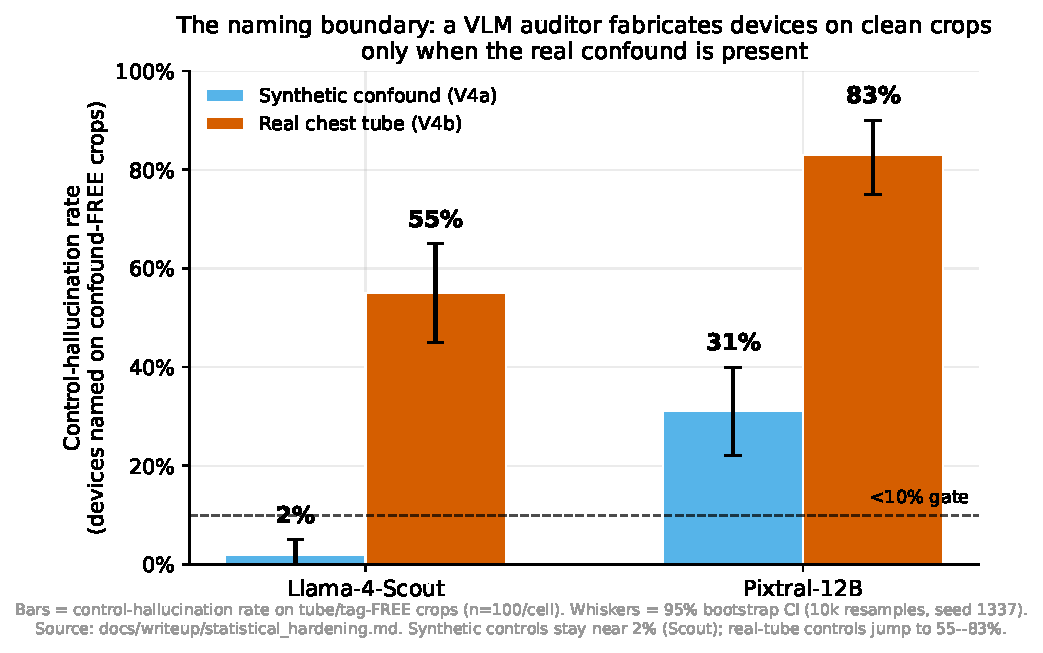
\includegraphics[width=0.9\textwidth]{figures/figure1_naming_boundary.pdf}
\caption{The naming boundary: control-hallucination (device named on a
confound-free crop) for each VLM on the synthetic confound versus the real
chest tube. The boundary is per-model, not a flat clean split:
Llama-4-Scout rises from 0.02 (synthetic) to 0.55 (real); Pixtral-12B rises
from 0.31 (synthetic) to 0.83 (real). Both fabricate a device on a majority
of clean control crops in the real-device setting; Pixtral already
fabricates on nearly a third of clean synthetic-setting crops. The $<$10\%
gate is cleared only by Scout on the synthetic confound.}
\label{fig:boundary}
\end{figure*}

\subsection{The failure is a property of general VLMs, not of one model}
It can be argued, however, that another VLM would not produce such negative results.
We performed the exact same procedure using 200 V4b crops, the same blind prompt,
and the same \texttt{names\_tube} matching tool on two separate VLM
families (Table \ref{tab:multivlm}).

\begin{table}[h]
\caption{Multi-VLM replication on V4b (real chest tube).}
\label{tab:multivlm}
\centering
\small
\begin{tabular}{|l|c|c|c|}
\hline
Model & Precision & Recall & Control-hallucination \\
\hline
Llama-4-Scout & 0.545 & 0.660 & 0.550 \\
Pixtral-12B & 0.494 & 0.810 & 0.830 \\
\hline
\end{tabular}
\end{table}

The Scout
repeat (0.550) matches the original V4b measurement (0.500) within
run-to-run API and decoding drift; Pixtral does considerably worse. Auditing
the raw text: the Scout fabricates particular devices on clean controls
(``endotracheal tube,'' ``central venous catheter''); Pixtral generates almost
identical boilerplate text (``linear radiopaque object\ldots appears to be a
medical device or foreign body'') for 83 out of 100 control crops.
The matcher is strict about positives,  will not match hedged
``linear artifact''  which tends to decrease recall in the correct
direction.

In other words, an auditor trained using off-the-shelf general VLMs would trigger
a false shortcut alarm on 55--83\% of the clean images (Scout 55\%, Pixtral
83\%). This is exactly what we wanted our precision-recall tradeoff gate
to identify, and which now we know is a property of all models. Bootstrap analysis (10,000 samples, seed 1337) shows that the gap between synthetic and real
models is significant for both models: the 95\% confidence interval on the
V4a minus V4b difference does not include zero (Scout $-0.53$ [$-0.63$, $-0.43$];
Pixtral $-0.52$ [$-0.64$, $-0.40$]), and
Fisher's exact rejects independence (Scout $p = 1.22\times10^{-18}$; Pixtral
$p = 7.56\times10^{-14}$).  The outcome is also independently verified using
HalluCXR, which finds that hallucination rates in six VLMs range between 61.9\%
and 82.3\% for 856 chest x-rays, with the most severe hallucination occurring
in normal images.

\subsection{What survives the naming failure}
\label{sec:results-5.3}
Mitigation, which does not rely on naming, works based on the actual confound. DFR
improves worst-group (pneumothorax without tube) accuracy from 0.67 to 0.79
(mean of 3 random seeds; single-run value is 0.83) whereas in-distribution
(pneumothorax with tube) accuracy remains 0.96 to 0.96 and the reliance gap
is narrowed from 0.29 to 0.17, without test-distribution labels. DFR and JTT
always do better than ERM with respect to all three seeds -- DFR worst-group
accuracy 0.790 $\pm$ 0.036 vs.\ ERM 0.672 $\pm$ 0.022, with difference of
approximately 12 percentage points which is larger than the spread within the
same methods themselves. We provide this effect-size analysis rather than a
statistical test: paired t-test at $n=3$ has zero statistical power and a
untestable assumption of normality, therefore no p-values are presented;
the pattern of results, both alternatives outperform ERM in each seed
by a large margin compared to the observed variance is the point,
not p-value derived from 3 points (Table \ref{tab:mitigation}).

\begin{table}[h]
\caption{Mitigation comparison: ERM, JTT, DFR on the real tube confound and
the synthetic tag confound (3-seed mean $\pm$ std).}
\label{tab:mitigation}
\centering
\small
\begin{tabular}{|l|l|c|c|c|}
\hline
Confound & Method & Worst-group & ID & Reliance gap \\
\hline
tube & ERM & 0.672 $\pm$ 0.022 & 0.959 $\pm$ 0.002 & 0.287 $\pm$ 0.025 \\
tube & JTT & 0.791 $\pm$ 0.047 & 0.940 $\pm$ 0.019 & 0.149 $\pm$ 0.031 \\
tube & DFR & 0.790 $\pm$ 0.036 & 0.964 $\pm$ 0.007 & 0.174 $\pm$ 0.029 \\
tag & ERM & 0.500 $\pm$ 0.000 & 0.940 $\pm$ 0.000 & 0.440 $\pm$ 0.000 \\
tag & JTT & 0.608 $\pm$ 0.018 & 0.531 $\pm$ 0.016 & $-0.077$ $\pm$ 0.025 \\
tag & DFR & 0.609 $\pm$ 0.022 & 0.603 $\pm$ 0.014 & $-0.006$ $\pm$ 0.024 \\
\hline
\end{tabular}
\end{table}

\begin{figure*}[!t]
\centering
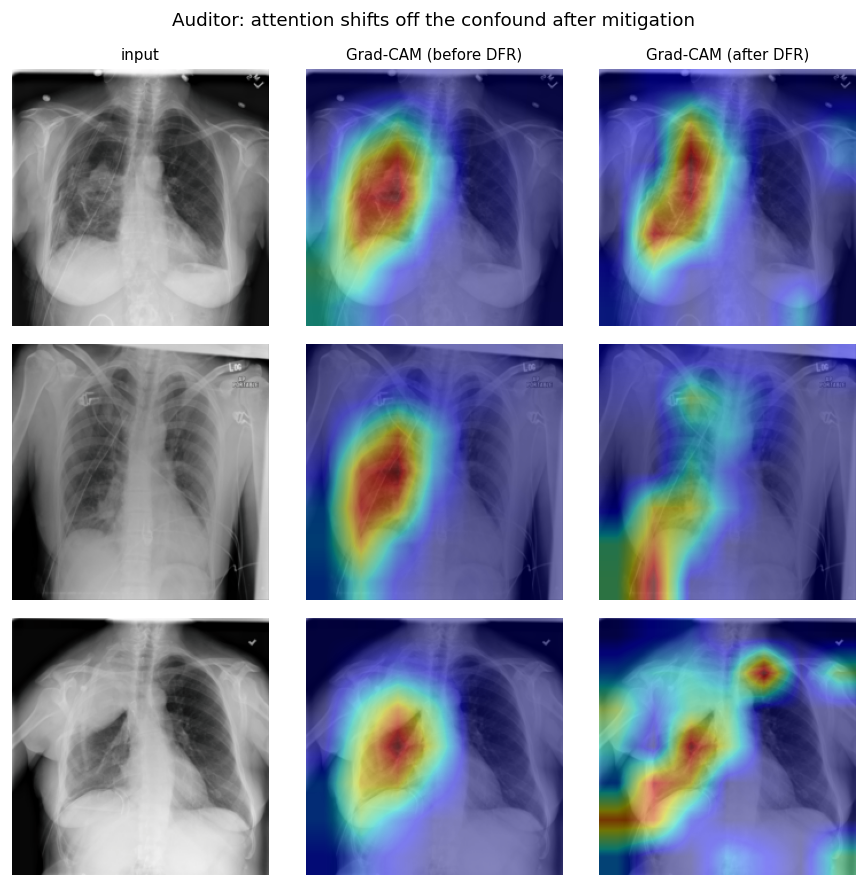
\includegraphics[width=0.9\textwidth]{figures/auditor_before_after_tube.png}
\caption{Before/after Grad-CAM on the real tube model, produced by a single
auditor command (detect$\rightarrow$mitigate). After DFR last-layer
retraining, attention broadens away from the confound-associated region
while in-distribution accuracy is preserved (0.96$\to$0.97 on this single
demo run) and worst-group accuracy rises.}
\label{fig:beforeafter}
\end{figure*}

In the synthetic tag experiment, the gap narrows (0.44 $\rightarrow$ 0.02) while in-distribution accuracy drops from 0.94 to 0.62. The linear probing done with the explicit intent of disproving the appealing interpretation that "the backbone is hollow" yielded probe AUC of 0.690  more than chance (0.50), but less than the baseline clean case (0.845).Dependence on shortcuts reduces, but does not impair,
the acquisition of core features, and the reduction depends on strength.

However, a real difference does exist that cannot be accounted for by the
shortcut. This comparison uses 8,000 image subsample of the full 25,600 image
NIH test split (intentionally limited due to the cost of computation in
the V6 cross-site runner (\texttt{run\_v6.py}'s \texttt{max\_per\_split=\{"test":
8000\}}, selected due to the stability of AUC at this size) – different from
the headline AUC of V1 test split AUC (0.8448) on all 25,600 images). On
this 8,000 image subsample, NIH AUC 0.842 drops down to PadChest AUC 0.650,
a difference of 0.192 (95\% CI [0.159, 0.225]). NIH sample ($n=8,000$)
and PadChest sample ($n=5,289$) are two disjoint sets without any overlap in
images or patients, thus their AUCs are bootstrapped independently (2,000
stratified resamples are drawn independently within each dataset) and the
confidence interval of the drop is the distribution of the difference between
the two independent samples per resample; this is the standard procedure for  difference between two independent samples, matching the magnitude
reported by Zech et al. -- a robust effect, not a borderline one. Supervised
Target Adaptation recovers $+0.082$  but this is fitting to last layer in
PadChest labeled data and will work regardless of a shortcut, thus does not
justify mitigation at all. The proper test, Zero-Shot Source Domain-Feature
Representation without using any target labels, produces $+0.005$ (95\% CI
[$-0.018$, $+0.028$], bootstrap method identical to the other two tests).
This interval does not contain a large recovery and contains zero, thus the
point estimate does not demonstrate any effect, but the interval is wide
enough to not rule out small-to-moderate effect (about $+0.03$ AUC): it is
underpowered null hypothesis, and we report it as such. The 0.192 AUC drop is
the distribution shift caused by something, and this experiment design cannot
tell what it is; possible causes include shortcuts, as well as scanner
differences, population differences, labeling pipeline differences, intensity
distribution residual and subset composition difference.

\section{Phase 5 Extension Experiments}
\label{sec:phase5}
After the V4b failure and pivot, five experiments were designed and run to
sharpen the V4b boundary -- i.e., to map why naming succeeds on a synthetic
confound but fails on a real device. All were run under the same validation
discipline: measure first, interpret second, no target outcome assumed.

\subsection{Naming-Difficulty Curve: Visibility vs.\ Hallucination}
Working hypothesis (pre-experiment): fabrication rises as the confound gets
fainter. We tested it directly by sweeping the synthetic tag's opacity
across $\{0.25, 0.5, 0.75, 1.0\}$ and re-scoring both models with the
unchanged pipeline ($n = 200$ crops per cell, 100 positive + 100 control),
reported in Table \ref{tab:opacity}.

\begin{table}[h]
\caption{Naming-difficulty (opacity) sweep.}
\label{tab:opacity}
\centering
\small
\begin{tabular}{|c|l|c|c|c|}
\hline
Opacity & Model & Precision & Recall & Control-hallucination \\
\hline
0.25 & scout & 0.600 & 0.030 & 0.020 \\
0.25 & pixtral & 0.420 & 0.210 & 0.290 \\
0.50 & scout & 0.963 & 0.520 & 0.020 \\
0.50 & pixtral & 0.588 & 0.400 & 0.280 \\
0.75 & scout & 0.978 & 0.900 & 0.020 \\
0.75 & pixtral & 0.556 & 0.400 & 0.320 \\
1.00 & scout & 0.978 & 0.900 & 0.020 \\
1.00 & pixtral & 0.626 & 0.520 & 0.310 \\
\hline
\end{tabular}
\end{table}

\textbf{Finding:} reducing visibility produces a recall cliff -- Scout's
recall collapses 0.90 $\to$ 0.52 $\to$ 0.03 between opacity 0.75, 0.5 and
0.25 -- while control-hallucination stays flat: ~0.02 for Scout and
~0.28--0.32 for Pixtral across every opacity level. Faintness makes the model
miss the confound; it does not make the model invent one.

\textbf{Interpretation:} this rules out visibility as the bridge from V4a's
0.02 hallucination to V4b's 0.50--0.83. Whatever separates the synthetic tag
from the real tube, it is not how hard the confound is to see. The revised
working hypothesis is that fabrication tracks the anatomical plausibility of
the confound category: a synthetic tag is never mistakable for anatomy at
any opacity -- it is either seen or not, with no ambiguous middle -- whereas a
real device sits inside a space of plausible near-misses (other lines,
catheters, vessels, fissures, rib edges) that a VLM's medical-image priors
can generate confident boilerplate about.

\subsection{Image-Independence: Is Fabrication Grounded?}
\label{sec:disc-6.2}
Working hypothesis (pre-experiment): the VLM is not reading the image at
all -- a live concern, since Lotfinia et al.\ show VLMs can answer
chest-radiograph questions from language priors without attending to the
image.

Test: three per-crop conditions scored against each model's own
unmodified-crop baseline description: occlude the relevant region, occlude
an equal-area irrelevant region, or swap in a different same-kind crop.
Verdict changes are broken down by direction: pos$\to$neg (named at
baseline, not named after) is consistent with grounding; neg$\to$pos (a new
device named after the edit) is fabrication merely relocated. All 12 cells
at $n = 100$ are reported in Table \ref{tab:occlusion}.

\begin{table*}[t]
\caption{Image-independence (occlusion/swap) study.}
\label{tab:occlusion}
\centering
\footnotesize
\begin{tabular}{|l|l|l|c|c|c|c|}
\hline
Dataset & Condition & Model & pos$\to$neg & neg$\to$pos & unchanged & rate \\
\hline
v4a & relevant & scout & 19 & 5 & 76 & 0.24 \\
v4a & relevant & pixtral & 25 & 22 & 53 & 0.47 \\
v4a & irrelevant & scout & 16 & 5 & 79 & 0.21 \\
v4a & irrelevant & pixtral & 27 & 24 & 49 & 0.51 \\
v4a & swap & scout & 8 & 8 & 84 & 0.16 \\
v4a & swap & pixtral & 27 & 23 & 50 & 0.50 \\
v4b & relevant & scout & 61 & 1 & 38 & 0.62 \\
v4b & relevant & pixtral & 66 & 5 & 29 & 0.71 \\
v4b & irrelevant & scout & 30 & 4 & 66 & 0.34 \\
v4b & irrelevant & pixtral & 13 & 2 & 85 & 0.15 \\
v4b & swap & scout & 20 & 21 & 59 & 0.41 \\
v4b & swap & pixtral & 17 & 17 & 66 & 0.34 \\
\hline
\end{tabular}
\end{table*}

\textbf{Methodology caveat:} the flat gray fill used to occlude the tag is
itself routinely described by the VLM as ``a gray rectangular object\ldots
artificial and not part of the patient's anatomy\ldots a label or marker'' --
language that trips the exact \texttt{names\_confound} rule the tag was
designed to trigger. Consequently, V4a's \texttt{relevant} numbers understate
true grounding, and the V4a-vs-V4b comparison is invalid for this question --
the measurement is biased toward \texttt{unchanged} for V4a in a way it is
not for V4b.

The evidence that carries the conclusion is the V4b-internal contrast. V4b's
matcher (\texttt{names\_tube}) requires device-specific vocabulary -- which a
flat gray rectangle does not resemble the way it resembles a generic
``artificial marker'' -- so its susceptibility to the artifact is far lower.
Within V4b, both conditions use the same matcher on the same dataset,
differing only in where the occluder lands: occluding the tube region drops
device-naming (pos$\to$neg 61/100 Scout, 66/100 Pixtral), while occluding an
equal-area irrelevant region drops it far less (30/100 Scout, 13/100
Pixtral). Device-naming tracks the tube pixels. ``V4b fabrication is pure
image-independent prior-emission'' is not supported. The reconciled
mechanism: the VLM carries a strong device-present prior and grounds it on
the salient region -- correctly reading a real tube when one is present, and
over-reading ambiguous normal anatomy as a device when none is. This is
prior-driven over-reading of an ambiguous salient region: neither blind
recitation nor clean perception.

\subsection{Specialist VLM: Over-Naming vs.\ Under-Naming Axis}
\label{sec:phase5-6.3}
\textbf{Question:} does a domain-specialized radiology VLM move the naming
failure boundary, or just shift which priors it emits?

\textbf{Finding 1: general VLMs over-name.} The V4b fabrication that
triggered the pivot was a general-VLM behavior: on tube-free controls,
Llama-4-Scout fabricates a device on 0.55 of clean crops and Pixtral-12B on
0.83. qwen2.5-vl-7b -- a larger general VLM -- over-names just as hard: its
V4b control-hallucination is 0.74. Over-naming is not an artifact of small
models; it persists at 7B on a fresh model family.

\textbf{Finding 2: specialist under-names, but structurally.} CheXagent-2-3B
does not answer in free text; it emits grounding tokens. Scored with a
grounding-aware matcher, it clears V4a's precision handsomely (precision
0.9663, recall 0.86, control-hallucination 0.03) but scores exactly
0.0/0.0/0.0 on V4b. This is not a perception failure: CheXagent produced a
grounded label on 100/100 V4b tube-positive crops. It is a taxonomy failure.
Its entire observed grounding vocabulary is \texttt{\{foreign object,
diaphragm, other lesion, artificial object, aortic enlargement,
mediastinal\}} -- no device-specific class exists anywhere in its output
space: nothing that says tube, catheter, line, drain, or wire. The
specialist can localize the tube and cannot name it, because ``name it as a
device'' is not an option its taxonomy affords.

This raises a natural follow-up: even without the vocabulary to say ``tube,''
did CheXagent's grounding boxes at least land in the right place? NEATX
provides no pixel bounding box for tubes (only the coarse L/R side label used
throughout this project), so a precise overlap check isn't possible, but a
side-check is: of the 100 V4b tube-positive crops, 88 have a single scorable
side (R: 59, L: 29); the other 12 are bilateral (\texttt{side='BOTH'} in
NEATX) and are excluded, the same way \texttt{peak\_on\_side} excludes them
elsewhere, since a bilateral annotation has no single correct half to check
a box against. Across those 88 crops, boxes labeled \texttt{foreign object}
or \texttt{artificial object} (22 total, its closest approach to flagging
something anomalous) land on the annotated side 14/22 (63.6\%) of the time --
nominally above the 50\% chance level, but a binomial test gives $p=0.14$
(95\% CI [0.44, 1.0]), not distinguishable from chance at this sample size.
Across all grounding boxes regardless of label (170 total, mostly
\texttt{diaphragm}), side accuracy is 51.8\% -- indistinguishable from chance.
This does not rescue the taxonomy-failure reading; it reinforces it:
CheXagent is not quietly localizing the tube under a euphemistic label, it
is not tracking the tube's location at all.

\textbf{Finding 3: caution on the over-clean reading.} ``Specialist
under-names, general over-names'' is the axis, but it is not the only axis,
and the general models are not uniformly safe wherever the specialist is
silent. Even on the easy synthetic V4a controls, fabrication is
model-dependent: Scout hallucinates on 0.02 of clean crops but Pixtral on
0.31 -- a per-model fabrication floor that has nothing to do with domain
specialization. The auditor's reliability therefore turns on the specific
model on both axes at once -- how much it over-names on clean crops and
whether its vocabulary can name the target at all.

\subsection{VLM-Independent Investigations}
Five investigations probe the robustness of the core results without
invoking the naming step. None is a headline; each either strengthens a
claim by an independent route or bounds an alternative explanation.

\subsubsection{Investigation 1: Severity-Stratified Tube Reliance}
Setup: stratify the 94 overlapping pneumothorax-positive test images at the
median bounding-box area. Within each tier, measure accuracy with vs.\
without the tube. Accuracy is perfect (1.0000) whenever a tube is present, at
any lesion size. Accuracy collapses when absent, at any lesion size:
low-severity gap 0.400, high-severity gap 0.4375. The gap is large in both
tiers, ruling out a pure disease-burden proxy. The study is underpowered
($n=16$--20/group) to distinguish true invariance from a real severity
effect; the invariance claim is withdrawn. What stands is that even
low-severity cases show a large gap -- the shortcut is device-keyed, not
disease-burden-keyed.

\subsubsection{Investigation 2: Canonical DFR Refit}
\label{sec:phase5-6.4.2}
Setup: tune regularization $C$ via 5-fold cross-validation, average weights
over 10 balanced draws. Table \ref{tab:canonicaldfr} reports the tube and
tag results.

\begin{table}[h]
\caption{Canonical DFR refit vs.\ standard DFR (tube and tag confounds).}
\label{tab:canonicaldfr}
\centering
\footnotesize
\begin{tabular}{|l|p{62pt}|c|c|c|}
\hline
Confound & Variant & Worst-group & ID & Gap \\
\hline
tube & before DFR & 0.6700 & 0.9575 & 0.2875 \\
tube & standard DFR & 0.8425 & 0.9650 & 0.1225 \\
tube & canonical DFR & 0.9275 & 0.9975 & 0.0700 \\
tag & before DFR & 0.5000 & 0.9397 & 0.4397 \\
tag & standard DFR ($C{=}1.0$) & 0.5927 & 0.5937 & 0.0010 \\
tag & canonical DFR ($C{=}0.001$) & 0.6813 & 0.6870 & 0.0057 \\
\hline
\end{tabular}
\end{table}

\textbf{Finding (tube):} the canonical variant strictly dominates the
standard one on all three metrics. The DFR result is a floor, not a ceiling
-- but the reported 0.79 (3-seed mean) is the number we defend most
strongly.

\textbf{Finding (tag):} standard DFR ($C=1.0$) causes a catastrophic ID
accuracy collapse (0.94 $\to$ 0.59); the gap nearly vanishes (0.001) but only
because the model is now near-random overall, not because confound reliance
was untangled. Canonical DFR ($C=0.001$, 10-draw) preserves the near-zero
gap (0.0057) while recovering some ID accuracy (0.687), still well below the
pre-DFR baseline (0.94). This is not a data-loading bug -- it is an
intentional construction that reveals a real limitation. Because the tag is
a synthetic, injectable marker rather than a naturally-varying device,
measuring both confound states requires building an untagged copy and a
synthetically re-tagged copy of the same validation images and concatenating
them -- the only way to construct all four \texttt{(confound, label)} groups
for a marker that can be painted onto any image at will
(\texttt{extract\_full\_val\_tag}, \texttt{canonical\_dfr.py}; the same logic
underlies V2's aligned/removed/flipped reliance-gap conditions). The
consequence is real: pairing each image with itself under both confound
states gives the logistic head no clean confound-vs-label axis to separate,
and it collapses toward a coin-flip regardless of $C$ or draw count. A
plausible complementary reading is feature dominance rather than pure
axis-indistinguishability -- at $p=0.95$ the backbone's representation is so
shaped by the tag that once the tag is decorrelated from the label by
construction, the remaining disease-relevant signal is too weak relative to
it to support accurate classification -- but this project did not separately
inspect feature magnitudes or head weights to adjudicate between the two
framings, so both are offered as consistent with the observed collapse
rather than either being independently confirmed. This is a boundary
condition of linear last-layer reweighting specific to paired-copy synthetic
confounds, not evidence that the pipeline is unreliable elsewhere -- but it
does mean the tag-DFR numbers above are uninterpretable as a measurement of
DFR's mitigation efficacy. The tube result, not the tag result, is the one
this project defends as a mitigation claim; the tag result stands only as a
pipeline-validation and cautionary data point.

\subsubsection{Investigation 3: Site-Projection Re-Decodability}
Setup: fit a hospital-detector probe on raw features. Then project out the
probed site direction and re-score disease AUC. Results: hospital detector
AUC 0.9993 (site is almost perfectly encoded); disease AUC before projection
0.6436; disease AUC after projecting out site 0.6436 ($\Delta$ 0.000);
site-probe AUC on projected features 0.9990 (site signal survives almost
completely).

\textbf{Finding:} site identity is redundantly encoded across many
directions. A rank-1 projection is insufficient to ablate site information;
a full subspace intervention would be required.

\textbf{Companion check:} label-free test-time adaptation recovers none of
the gap. Two standard TTA methods were run on the frozen V1 model against
PadChest, touching no target labels: BN-adaptation (re-estimating BatchNorm
running statistics on the target images) moves AUC by $-0.004$, and TENT
(entropy-minimizing the BN affine parameters) actively harms it ($-0.122$,
collapsing toward chance). TENT was designed around multi-class categorical
entropy; on this architecture's single-logit binary head, the entropy being
minimized is a degenerate special case that can drive the logit toward an
extreme, miscalibrated value rather than genuine adaptation. This result is
consistent with that known architecture mismatch specifically, not a general
claim about TENT's suitability for chest-radiograph adaptation in properly
multi-class or calibrated setups. Together with the site-projection null
above, this rules out the two mechanisms one would reach for first -- a
disease head riding a decodable site signal, and a covariate shift
correctable by cheap label-free adaptation -- leaving most of the 0.192 gap
as genuine, unattributed distribution shift.

\subsubsection{Investigation 4: Label-Free OOD-Gap Attribution (Tag Source-DFR)}
Setup: generalize the zero-shot source-DFR test from the tube confound to
the synthetic tag. Mitigate tag reliance on NIH (zero PadChest labels), then
evaluate on PadChest (Table \ref{tab:tagsourcedfr}).

\begin{table}[h]
\caption{Label-free OOD-gap attribution: tag source-DFR.}
\label{tab:tagsourcedfr}
\centering
\small
\begin{tabular}{|l|c|}
\hline
Metric & Value \\
\hline
NIH test AUC (tag model) & 0.7407 \\
PadChest AUC before mitigation & 0.6345 \\
PadChest AUC after tag source-DFR & 0.5520 \\
Zero-shot change & $-0.0825$ \\
\hline
\end{tabular}
\end{table}

\textbf{Finding:} tag source-DFR does not improve PadChest AUC; it makes it
substantially worse. The tag shortcut is so dominant that the feature space
has largely collapsed to encoding the tag rather than disease. This
asymmetry (vs.\ the tube's $+0.005$ null) is consistent with the tag being a
far more complete representation override. Synthetic confounds prove the
method but systematically overstate the severity of the phenomenon relative
to real ones.

\section{Discussion}
\label{sec:discussion}
The paper's spine is a boundary: blind, general-purpose VLM naming works
where a shortcut is unmistakable and fails -- by fabrication -- where a
shortcut is a plausible member of a familiar category. The two mechanism
experiments locate which axis the boundary runs along. It is not
visibility: faintness produces a recall cliff, not a hallucination cliff
(\S6.1). It is plausibility. A synthetic corner tag is never mistakable for
anatomy at any opacity, so the model either sees it or does not; a chest
tube lives among lines, catheters, vessels, fissures, and rib edges that a
device-primed VLM can write confident boilerplate about. \S6.2 then rules
out the deflationary reading that the VLM ignores the image: device-naming
tracks the tube pixels (occluding the tube drops naming roughly twice as
much as occluding an equal-area irrelevant region). The failure is therefore
neither blind recitation nor clean perception -- it is prior-driven
over-reading of an ambiguous salient region.

We frame the failure as an over-name/under-name axis, because the two
directions carry different costs for an auditor. Under-naming (a miss)
degrades gracefully -- \S6.1 shows that as the confound fades the model
simply stops naming it, and the recall bar is set below precision precisely
to tolerate this. Over-naming (fabrication) is the dangerous direction: a
tool that invents a chest tube on a clean radiograph will send a clinician
chasing a shortcut that is not there, and at 55--83\% on clean crops it would
do so on a majority of images. This is why the design made
control-hallucination a gate rather than a reported statistic, and why the
honest verdict is that off-the-shelf general VLMs are not safe as blind
auditors of clean images without such a gate. That the boundary is
per-model rather than a flat clean split (Scout fabricates on 2\% of
synthetic controls but Pixtral on 31\%) sharpens rather than softens the
conclusion: even in the ``easy'' synthetic setting, one of two general
models already fails the gate.

What survives the naming failure matters for how the contribution should be
read. The mitigation result is real, defensible, and -- by construction --
independent of the broken naming step: no method in the mitigation path
imports the VLM module, so the naming-off ablation is not a separate
experiment but a property of the code. DFR recovers worst-group accuracy on
the real tube from 0.67 to 0.79 (3-seed mean) with in-distribution accuracy
preserved and no target-distribution labels, and two independent methods
agree well outside seed variance. We are deliberate about the headline
number: 0.79 is the 3-seed mean; the single-draw 0.83 appears only when
explicitly labeled as such, because reporting the luckier draw as the result
would be the same over-claiming the paper's method is designed to catch. The
synthetic tag supplies the cautionary companion -- a pure shortcut at
$p=0.95$ so thoroughly overrides the representation that removing it leaves
too little disease signal behind, which is exactly why synthetic confounds
prove the method but overstate the phenomenon.

The cross-site result is where we most resist the tempting story. There is
a real 0.192 US-to-Spain AUC drop, Zech-magnitude, and it would be easy to
present the loop as ``validated cross-site.'' It is not. The supervised
recovery ($+0.082$) uses PadChest labels and would help with no shortcut
present; the honest zero-shot source-DFR test -- reduce the known tube
shortcut on NIH only, touch no target labels -- returns $+0.005$ (95\% CI
[$-0.018$, $+0.028$]): a point estimate indistinguishable from zero. Reducing
a known source shortcut did not measurably narrow the cross-site gap in this
test, so the gap is distribution shift this design cannot attribute to the
shortcut -- while acknowledging the test's power to detect a modest effect,
had one existed, was limited. The representation-level controls corroborate
rather than rescue this: site identity is almost perfectly decodable (AUC
0.9993) yet the frozen disease head does not read it ($\Delta$ 0.000 after
projecting site out), so the two mechanisms one reaches for first -- a head
riding a site signal, and a covariate shift correctable by label-free
adaptation -- are both bounded near zero, leaving most of the gap genuinely
unattributed. The clinically load-bearing consequence is that ``fix the
known shortcuts'' is not sufficient due diligence before cross-site
deployment.

Finally, honest scope. This is one pathology (pneumothorax), one primary
corpus (NIH) with one second site (PadChest), one real device confound
(chest tube) with non-expert labels, and general (not specialist) VLMs. The
two mechanism experiments bound the boundary on the visibility and
image-grounding axes but do not map it along the plausibility axis the
mechanism implicates -- we know naming works on an unmistakable marker and
fails on a subtle device, not where in between it turns over. The
pre-registered stopping rule governed the gate decision itself -- a V4b
failure after a V4a pass triggered an immediate, reported pivot rather than
iteration on that decision -- but it did not foreclose a cheap follow-up
ablation (abstention prompting), which was designed and coded but not
executed before this writeup. The boundary is therefore characterized, not
mapped, partly by design and partly because that follow-up remains unrun.

\section{Limitations}
\label{sec:limitations}
\textbf{Single pathology, single primary corpus.} Every result concerns
pneumothorax on NIH ChestX-ray14 and its cross-site evaluation on PadChest.
The mechanism proposed in \S\ref{sec:phase5} -- fabrication driven by the
anatomical plausibility of the confound category -- predicts that other
device-adjacent pathologies would behave similarly, but this is a
prediction, not a measurement.

\textbf{Non-expert ground truth for the real confound.} NEATX's chest-drain
annotations come from two data-science students, not radiologists, with
``moderate to almost perfect'' agreement against expert labels reported in
the source paper. This is adequate for inducing a training-time enrichment
signal and defining a mitigation target, but it is a noisier ground truth
than a radiologist-drawn segmentation would provide for V4b's
precision/recall scoring specifically.

\textbf{The auditor's own VLM component was not tested for pure
image-independence in V4a.} Lotfinia et al.\ show VLMs can answer CXR
questions from language priors without attending to the image. \S6.2
addresses this and does not support blind recitation as the explanation of
V4b (device-naming tracks the tube pixels), but a clean counterfactual-image
test on V4a specifically -- free of the flat-gray-occluder artifact documented
in \S6.2 -- remains the most direct follow-up. That same occluder artifact
also means the V4a-vs-V4b grounding comparison in \S6.2 is not directly
available: V4a's \texttt{relevant}-occlusion numbers are contaminated by the
occluder itself tripping the \texttt{names\_confound} matcher, so the
image-independence conclusion rests entirely on the V4b-internal contrast
(relevant vs.\ irrelevant occlusion, same matcher, same dataset). This is
sufficient to support the grounding claim made, but it means no experiment
in this project directly compares V4a's and V4b's degree of grounding to
each other.

\textbf{The V4b matcher's false-negative rate has been audited;} a small,
quantified vocabulary gap exists but does not change the verdict. A manual
audit of all 34 V4b recall misses (mirroring the V4a 23-miss audit) found: 2
of 34 (5.9\%) are confirmed matcher/regex bugs -- the VLM explicitly and
unambiguously identified a device (``\ldots appear to be wires, likely from
an ECG or other monitoring device''; ``\ldots likely to be medical devices,
specifically the patient's ECG leads''), but the \texttt{names\_tube} regex
matches singular ``wire''/``lead''/``medical device'' and not their plural
forms. 1 of 34 shows the VLM detecting a real but different device (a
``pacemaker or implantable cardioverter-defibrillator,'' not the annotated
chest tube). The remaining 31 of 34 (91\%) are genuine VLM perception
failures -- explicit ``no artificial/foreign objects, normal anatomy''
statements, or tube-like linear structures misattributed to ribs, the
imaging grid, or clothing. Correcting the two confirmed regex bugs would
raise V4b recall from 0.66 to at most 0.68 -- still below the 0.70 gate, so
the FAIL verdict is unchanged. The control-hallucination result (0.50, the
metric that actually drove the pivot) is unaffected either way, since
control-hallucination requires the matcher to fire on a negative crop, not
to miss on a positive one, and this audit only examined misses.

\textbf{Two-site validation; V6 causal attribution narrowed but not closed.}
Two sites are two points, not a trend. The cross-site drop (0.192) is real
and Zech-magnitude, and the \S6.4.3 controls rule out two candidate
mechanisms -- a disease head riding a decodable site signal ($\Delta$ 0.000)
and label-free covariate shift correctable by standard test-time adaptation
(BN-adaptation $-0.004$; TENT $-0.122$, actively harmful). But most of the
gap remains genuine, unattributed distribution shift. Candidate causes this
design cannot separate include scanner and acquisition differences,
population differences, the two datasets' different label-generation
pipelines (NIH's NLP-only labeler vs.\ PadChest's NLP-plus-manual process),
residual intensity artifacts despite the 8-bit fix, and the composition of
the 573-positive/7,000-negative working subset. A third site would turn two
points into a trend; the design accommodates one without rework, but we did
not run it.

\textbf{Single-GPU scale; single-seed sweep.} All training ran on one
consumer GPU (RTX 3050, 6GB), which shaped batch size (16, after an OOM at
32), resolution (224px, standard for this literature), and the decision to
work with subsets (most visibly the 7,572-image PadChest working set). The
correlation sweep carries one training seed per point; its trend (monotone
reliance growth) is clear, but individual point values could shift under a
different seed. The 3-seed baseline table is the result we defend most
strongly on variance grounds.

\textbf{The difficulty boundary is bounded on one axis, unmapped on the
others.} \S6.1 rules out visibility as the axis along which naming degrades
into fabrication, and the multi-VLM replication (\S5.2) closes the ``a
different model would fix it'' escape hatch for general-purpose VLMs (55\%
and 83\% fabrication on clean crops). What remains open is where between an
unambiguous synthetic marker and a subtle real device the boundary sits
along the plausibility axis, and whether prompt design, crop resolution, or
abstention/confidence mechanisms shift it. An abstention-prompt ablation
targeting exactly this was designed and implemented but not executed before
this writeup; we report it as built-but-unrun rather than as a considered
decision not to attempt a rescue.

\textbf{Interpretive claims corrected mid-project.} Two claims were written
before the control that tests them existed, and both were withdrawn once it
was run: ``the pure-shortcut backbone is hollow'' (falsified by the linear
probe: AUC 0.690, above chance 0.50) and ``mitigation validated across three
settings'' (falsified by the zero-shot source-DFR null: $+0.005$, after the
$+0.082$ ``recovery'' was correctly re-identified as supervised target
adaptation). We report both, because the failure mode they share --
asserting an interpretation the experiment does not license -- is the same
one this project's method is designed to catch in a classifier.

\section{Conclusion}
\label{sec:conclusion}
We set out to build an auditor that detects, names, and mitigates a spurious
shortcut in a chest X-ray classifier, and we ran it under a validation-gated
discipline that let each stage's claim stand or fall on a pre-registered
threshold. Detection, localization, and mitigation transfer from a
synthetic confound to a real chest-tube confound: reliance is measurable,
attributable, and reducible -- worst-group accuracy on untreated (tube-free)
pneumothorax rises from 0.67 to 0.79 with no target labels, on a step that
provably never touches the VLM. The naming stage does not transfer. Blind,
general-purpose VLM naming passes at near-ceiling on an unmistakable
synthetic marker and fails on the real device by fabrication, inventing
chest tubes and catheters on a majority of clean radiographs -- a cross-model
failure, corroborated by independent benchmarks, that our control-hallucination
gate was built to catch and did. And the real cross-site drop we measured
is distribution shift we could not attribute to the shortcut, not a
mitigation success.

The contribution we stand behind is therefore not ``an auditor that names
shortcuts,'' but a mapped boundary of where that ambition currently breaks
and a defensible mitigation result that survives the break. Blind VLM
naming is a bounded capability -- trustworthy for salient, unambiguous
shortcuts, unsafe as a blind auditor of clean images without a false-alarm
gate. The most useful thing a capstone can do with a failed critical gate is
report it precisely, characterize why it fails, and show what still works
around it. That is what this project does: an honest negative result on
generative-model-free shortcut naming, wrapped in a mitigation and
cross-site study that neither overstates the recovery nor hides the
failure. The natural next steps -- a radiologist-grade real-confound corpus
for re-scoring the gate, a specialist-VLM arm to test whether radiology
fine-tuning moves the boundary, and a third site to turn two cross-site
points into a trend -- are all accommodated by the confound-agnostic design
without rework.

\section*{Ethics and Data/Code Availability}
This study used publicly available, de-identified datasets (NIH
ChestX-ray14, PadChest, NEATX). No patient-identifiable information was
accessed; institutional review was not required for secondary analysis of
public data. Code, configuration files, and prediction manifests for the
reported experiments are available upon reasonable request to the authors.

\appendices

\section{Reproducibility and Compute Cost}
\subsection{Configuration and Environment}
Every run is config-driven (typed YAML with inheritance and CLI overrides),
fixed-seeded, and logged to a timestamped directory. Dataset paths are
configuration values; no image or checkpoint is version controlled. The
codebase is organized into confound-agnostic modules with 128 passing
tests.

Python version: 3.9.13. PyTorch + CUDA: torch 2.4.0 on CUDA 12.1, timm
(vision models). Hardware: RTX 3050 6GB (Windows 11). Reproducibility:
\texttt{git rev-parse HEAD} recorded in every run; all random seeds fixed
(numpy, torch, Python).

\subsection{Compute Cost}
Extracted from \texttt{run.log} timestamps in experiment directories (Table
\ref{tab:compute}).

\begin{table}[h]
\caption{Local compute cost by run.}
\label{tab:compute}
\centering
\small
\begin{tabular}{|p{140pt}|c|}
\hline
Run & Wall-clock \\
\hline
V1 training (DenseNet-121, 5 ep, full split) & 45.1 min \\
V2 shortcut training & 34.2 min \\
V3 Grad-CAM attribution (200 images) & 21.1 min \\
Phase 3 baselines (ERM/JTT/DFR $\times$ 3 seeds $\times$ 2 confounds) & 16.6
min \\
V5 DFR fit (single run) & 1.4 min \\
V6 cross-site eval & 2.6 min \\
\hline
\textbf{Total (core reported runs)} & \textbf{~2.0 GPU-hours} \\
\hline
\end{tabular}
\end{table}

Not included: correlation-strength sweep (5 training runs, ~2.5--4 hours),
V4 crop export (much smaller), exploratory/failed runs. Total estimated
local compute: 2--6 GPU-hours on a single consumer laptop GPU.

\subsection{VLM API Calls}
Counted from \texttt{predictions*.jsonl} line counts (Table \ref{tab:apicalls}).

\begin{table}[h]
\caption{VLM API call counts by study.}
\label{tab:apicalls}
\centering
\small
\begin{tabular}{|l|c|}
\hline
Study & Calls \\
\hline
V4a + V4b canonical & 400 \\
Multi-VLM replication & 400 \\
Opacity sweep (Exp 1) & 1,600 \\
Occlusion study (Exp 2) & 1,200 \\
Specialist arm (Exp 3) & 2,000 \\
\hline
\textbf{Total} & \textbf{5,600 free-tier calls} \\
\hline
\end{tabular}
\end{table}

All against free-tier APIs (Groq, Mistral La Plateforme, Google AI Studio);
zero marginal cost, no generative model or fine-tuning at any point.

\section{Statistical Hardening}
Post-hoc bootstrap statistics over existing prediction files (no new runs).

\subsection{Control-Hallucination Rate per Cell}
\begin{table}[h]
\caption{Control-hallucination rate per cell, with bootstrap 95\% CI.}
\label{tab:halluccell}
\centering
\small
\begin{tabular}{|l|l|c|c|c|}
\hline
Dataset & Model & Flagged/$n$ & Point est. & 95\% CI \\
\hline
V4a & scout & 2/100 & 0.02 & [0.00, 0.05] \\
V4b & scout & 55/100 & 0.55 & [0.45, 0.65] \\
V4a & pixtral & 31/100 & 0.31 & [0.22, 0.40] \\
V4b & pixtral & 83/100 & 0.83 & [0.75, 0.90] \\
\hline
\end{tabular}
\end{table}

\subsection{V4a-vs-V4b Gap, per Model}
\begin{table}[h]
\caption{V4a-vs-V4b control-hallucination gap per model.}
\label{tab:gapmodel}
\centering
\small
\begin{tabular}{|l|c|c|c|}
\hline
Model & Gap (V4a$-$V4b) & 95\% CI on diff. & Fisher's exact $p$ \\
\hline
scout & $-0.53$ & [$-0.63$, $-0.43$] & $1.22\times10^{-18}$ \\
pixtral & $-0.52$ & [$-0.64$, $-0.40$] & $7.56\times10^{-14}$ \\
\hline
\end{tabular}
\end{table}

For both models, the 95\% bootstrap CI on the V4a-minus-V4b
control-hallucination difference excludes 0, and Fisher's exact test rejects
independence at the 0.05 level. The gap is statistically significant.

\textbf{Methodology:} non-parametric bootstrap, percentile method, 10,000
resamples, seed 1337. Gap bootstrapped directly (V4a and V4b resampled
independently per resample).

\section{Decision Log (abbreviated from PROGRESS.md)}
\begin{itemize}
\item \textbf{2026-07-07} -- Framework \& compute: PyTorch + timm
(DenseNet-121 @ 224px), local RTX 3050 6GB, AMP on, batch-size tuned.
\item \textbf{2026-07-08} -- V1 PASS: full-data test AUC 0.8448. Root-caused
CUDA memory failure to VRAM peak on AdamW; fixed by batch\_size 32$\to$16.
\item \textbf{2026-07-08} -- V2 PASS: reliance gap 44pp. acc\_removed landing
at 0.500 matches pure-shortcut fingerprint pre-validated before run.
\item \textbf{2026-07-08} -- V3 PASS: Grad-CAM peak-in-tag-box 100\% on
tagged positives vs.\ 0.5\% on untagged controls.
\item \textbf{2026-07-08} -- V4a PASS (CRITICAL GATE): Llama-4-Scout via Groq
named synthetic tag, P 0.978 / R 0.90 / halluc 0.02. Keyword matcher
corrected during scoring after auditing all 23 original misses.
\item \textbf{2026-07-08} -- V4b FAIL $\to$ PIVOT: real chest-tube confound.
Detect/localize succeeded (gap 28.75pp). Naming failed: P 0.57 / R 0.66 /
halluc 0.50. Llama-4-Scout fabricates devices on 50/100 tube-FREE controls
(47 of those 50 audited as explicit, genuine hallucination, not matcher
error). Pivot executed: auto-naming dropped; reframe as
detect$\to$localize$\to$mitigate without naming claim.
\item \textbf{2026-07-09} -- V5 PASS (DFR): REAL tube confound: worst-group
0.67$\to$0.79 (3-seed mean; a single-draw run gives 0.83), ID
0.96$\to$0.96 (3-seed mean). Synthetic tag ($p=0.95$): gap closes but ID
collapses 0.94$\to$0.62. Linear probe (AUC 0.690) shows backbone is
degraded, not hollow.
\item \textbf{2026-07-09} -- Phase 3: ERM/JTT/DFR baselines (3-seed table),
naming-off ablation, correlation-strength sweep (monotone gap vs.\ $p$),
GroupDRO skipped.
\item \textbf{2026-07-10/11} -- V6: NIH 0.842 $\to$ PadChest 0.650 (drop
0.192). Supervised adapt $+0.082$. Zero-shot source-DFR $+0.005$ (null).
Drop is distribution shift, not shortcut-driven.
\item \textbf{2026-07-11} -- CO1-CO4 writeup complete. Literature re-search,
novelty framing. Two corrected claims (hollow-shortcut, cross-site
mitigation).
\item \textbf{2026-07-14--15} -- Phase 5 Exp 1--3: opacity sweep, occlusion
study, specialist VLM (over-name/under-name axis).
\item \textbf{2026-07-16--18} -- Phase 5 Investigations 1--4:
severity-stratified gap, canonical DFR, site-projection, label-free
OOD-gap attribution.
\end{itemize}
All experiments complete. Capstone writeup assembled.

\section*{Acknowledgment}
Data-use credits: NIH ChestX-ray14, PadChest, NEATX. No specific funding is
asserted by this draft.

\bibliographystyle{IEEEtran}
\begin{thebibliography}{00}

\bibitem{zech2018} J. R. Zech \emph{et al.}, ``Variable generalization performance of a deep learning model to detect pneumonia in chest radiographs: A cross-sectional study,'' \emph{PLoS Medicine}, vol. 15, no. 11, 2018.

\bibitem{degrave2021} A. J. DeGrave, J. D. Janizek, and S.-I. Lee, ``AI for radiographic COVID-19 detection selects shortcuts over signal,'' \emph{Nature Machine Intelligence}, vol. 3, pp. 610--619, 2021.

\end{thebibliography}
\EOD

\end{document}
